\documentclass{amsart}
\usepackage[pdftex]{graphicx}

\title{Modeling Intervention Strategies for United States TB Control}
\begin{document}
\maketitle

\section{Introduction}
Epidemiological models allow public health professionals to predict and analyze
disease dynamics and intervention effectiveness. The most common examples of
such models are compartmental differential equation models, in which the
population is split between several possible health states, with flow between
each state given according to deterministic differential equations. In 2012, 
Hill, Becerra, and Castro implemented a compartmental
differential equaiton model of tuberculosis (TB) in the United States (US).
Their model utilized five health states and two subpopulations, US-born (USB)
and foreign-born (FB) for a total of 10 compartments. They used this model to
evaluate several possible intervention strategies, and ultimately conclude that
though increasing LTBI treatment was a good intervention strategy, the US was
unlikely to meet their stated goal of elimination of TB in the US by 2100. In
this work, the Hill model was extended in several key ways. First, additional
tracking capabilities were added to the Hill model, such that it can now report
further granularity in the disease dynamics. Further, economic components were
added to the model in order to project the US health care system (HCS) costs due
to TB given our current policy as well as for various interventions. Finally, a
population level, agent based implementation of the Hill Model was created, in
order to validate the Hill Model against the natural stochasticity present in
real world disease spread. 

\section{Background}

\subsection{The Hill Model}
A flowchart representation of the Hill Model is shown in Figure 1.  Each compartment
represents a different possible health state with respect to TB for every 
US-born or foreign-born individual, and arrows between different compartments
represent possible transitions between states.  Individuals also leave the model 
from all compartments due to natural death, which is left out of the figure for clarity.  \\

\begin{figure}
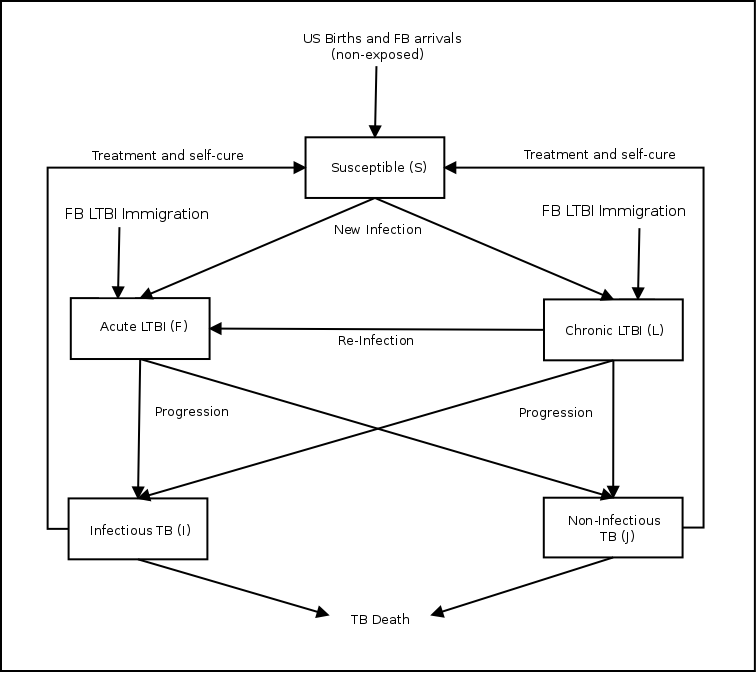
\includegraphics[scale=0.25]{figures/HillModelFlowChart.png}
\end{figure}

The majority of USB and FB individuals fall into the Susceptible (S) category, which includes everyone
who is uninfected and has not been exposed to TB.  After exposure to an individual
with TB, a person in the Susceptible compartment can develop Latent TB Infection (LTBI) and changes
health states to either the Acute LTBI (F) or Chronic LTBI (L) compartment.  Latently
infected individuals are not infectious, but have some risk of developing active TB infection
over time.  However, the rates of disease progression are not equal, and individuals in the
Acute LTBI compartment have a higher risk of developing active TB than those in
the Chronic LTBI compartment.  Individuals in the Chronic LTBI compartment
may also be exogenously re-infected and transition to the Acute LTBI compartment.  \\

Latently infected individuals may progress to one of two active TB states: Infectious TB (I) or 
Non-Infectious TB (J).  Individuals in both compartments have an increased risk of death from
active TB infection, but only individuals in the Infectious TB compartment are contagious.  
In addition, individuals in all of the infected compartments (F, L, I, J) may be treated or self-cure
themselves of their respective TB health condition.  However, in the model, treatment or self-cure from TB
does not grant immunity, and all healthy individuals are grouped in the Susceptible compartment
and may be re-infected at a later time.  \\

\section{Methods}
\subsection{Basic Implementation}
Both the basic Hill Model and this extended Hill Model were implemented in
\texttt{R} as a system of differential equations, which were solved via the
$\texttt{lsoda}$ routine. The systems of differential equations used in the Basic
Hill Model and the extended Hill Model to capture basic disease dynamics are
shown below in Figure 2 and Figure 3 respectively. In the extended Hill model,
more differential equations were implemented to add additional tracking and
economic modeling. These equations are detailed in the appendix. 

\begin{figure}
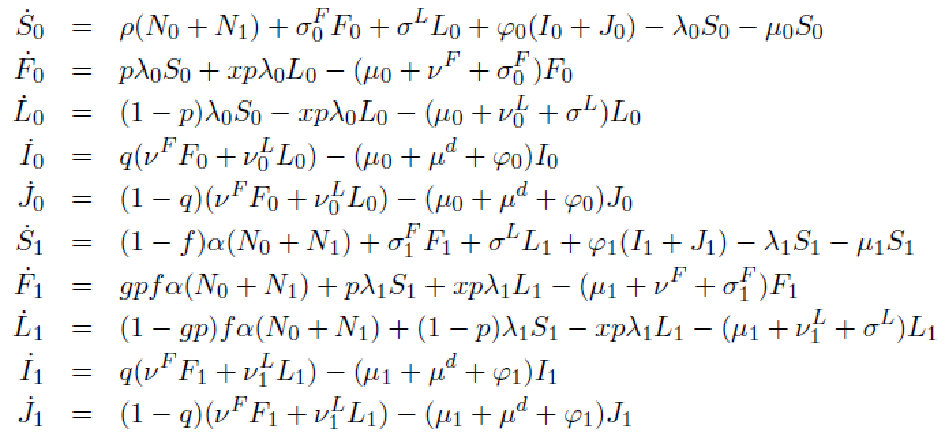
\includegraphics[scale=0.75]{figures/BasicHillEquations.pdf}
\end{figure}

The vector variables $S_{0}, F_{0}, L_{0}, I_{0}, J_{0}$ contain the number of
US-born individuals in the S, F, L, I, J compartments respectively, whereas $S_{1},
F_{1}, L_{1}, I_{1}, J_{1}$ contain foreign-born individuals.  $N_{0}$ and
$N_{1}$ are the total populations of US-born and foreign-born individuals.
The constants $\rho$ and $\alpha$ are birth rates, while $\mu_{i}$, and $\mu_{d}$ are death rates.  
A complete list and descriptions of all constants used in the model can be found in the appendix.

\subsection{Additional Tracking Capabilities}
In order to refine the tracking capabilities of the
Hill Model, the original differential equations used to describe TB spread were
separated into their component parts and each section was tracked separately.
These components were made into compartments, tracked by differential equations
detailed in the appendix. These equations allowed the model to track the total
number of TB cases, TB deaths, and  natural deaths. Further, the model tracks,
the sourced cost on the US HCS. Progressions into
active TB due to activations of LTBI or exogenous infection were tracked,
allowing for sourced incidence data to be generated. The entering cases of LTBI
(acute or chronic) were also tracked. In the case of intervention testing, the
number of cured cases of entering LTBI and the number of untreated entering LTBI
were both tracked. Cured cases of LTBI entering, TB deaths, total TB cases, and
total cost were also tracked discounted at 3\% annually. This discounting was
converted to a continuous differential equation for use within the model. In
general, incidence data is calculated in the same way in the extended hill as it
was in the basic Hill.

In addition, estimations of the basic reproductive number of FB or USB active,
infectious TB cases were made from a theoretical and an experimental
perspective. Experimental data were calculated by reducing the initial
population of FB or USB active, infectious TB cases by one and allowing the
model to progress otherwise as normal. The decreased number of total TB cases
seen details how many infections can be thought to be due to one infected
individual in the given population.

From an experimental perspective, the spread of TB was thought to be a geometric
series. If one infectious individual infects $x$ people annually, over the
course of $N$ years the total number of infections caused by this individual can
be approximated by the geometric series of $N$ terms with rate $x$ and initial
term $1$. In this case, $N = 100$, and the ratios for FB infectious individuals
and USB infectious individuals were obtained from RATIO CITATION COLIN. 
\subsection{Economic Modeling}
When tracking the economic implications of current US TB load and various
intervention strategies, active TB costs were given by \$14,000. This cost is
the weighted mean of the costs of cases requiring hospitalization (happening
49\% of the time) and cases not requiring hospitalization (51\%). These data
were found in DYLAN COST STUDY CITATION. LTBI treatment costs were given by
\$468.00. These data were based on the cost of a successfull treatment, given by
DYLAN COST STUDY CITATION, as well as adherence and efficacy data found in
ADHERENCE CITATION.

From these estimated cost per treatment, total costs were obtained by assuming
that every patient with active TB in the US is treated at full price, though the
treatment may fail. As individuals with active
TB are charged upon entry to the active TB compartment, the model can also
accurately estimate sourced US HCS cost data. Cost data were separately tracked
due to incoming active TB costs stemming from activation of LTBI vs exogenous
reinfection. These data were modelled as additional compartments and also solved
by $\texttt{lsoda}$. For LTBI treatment cost, treatment was
charged upon leaving the LTBI compartment due to the cumulative self-cure and
treatment rate given in the Hill Model. The fraction of these indviduals who
leave this compartment due to self cure was assumed to be zero. Given the
uncertainty in measurments of LTBI treatment cost, extensive sensitivity
analysis was performed on this parameter relative to final cost outcomes. In
addition to US HCS cost, the system was implemented so as to also track
projected intervention implementation cost, given user-inputted parameters
relating to various possible intervention cost strategies. The extended Hill
Model was used to track the effect of many interventions tested by the Hill
Model. In particular, the intervention strategy of curing entering cases of LTBI
proved very promising and elimination year, final cost, and cost per case
averted were tracked for various levels of entering LTBI cure rate. The
interventions were implemented so as to take effect during the year 2013 and run
to 2100. The numerical DE solver $\texttt{lsoda}$ used was run with a time step
of $0.8$. Sensitivity analysis was performed on this parameter and reducing the
time step was shown to have minimal effect on final size or cost values.

\subsection{Agent Based}
The population level agent based model was implemented in several ways. Early
implementations were built in \texttt{Netlogo} and \texttt{Java}, but final
implementations were constructed in $\texttt{C++}$. An implementation was made
that tracked the hill model exactly, up to still including the Acute Latent
compartment in the model. Probabilites of agent progression between various
health states were computed given rates in the hill model and a variety of
approximations. The model maintained scaled individual records for every
individual with LTBI, with susceptible individuals not modelled as agents.
Instead, a binomial distribution was used to probabilistically pick the number
of new infections each time step. Similarlly, immigration was also handeled
outside of the agent-based modelling. The final size standard deviation and
distribution data was collected via 2160 (MINUS SOME) runs with each agent in
the model truly representing one infected individual and a time step of $0.01$.
These data were analyzed in $R$. This model was also made to track deaths, total
TB cases, and infection sources. This data were consistent with the
deterministic model, and not reproduced in this write-up. 

Further implementations of the \texttt{C++} model were made that deviated from
the basic Hill Model. Specifically, the acute latent compartment in the basic
Hill Model is a vestigal necessity of compartmental modeling and not reflective
of the biology of tuberculosis, and an agent based model was implemented that
more closely respects the biology of tuberculosis. Results from this model or
the strict Hill model did not differ significantly. 
\section{Results}

\subsection{Basic Population Breakdown}
The additional tracking capabilities offered several key insights into US TB
dynamics. Figure INSERT FIGURE HERE shows the yearly incidence of US TB, broken
down into infection source. It can be seen that the majority of the US TB load
is driven by activations of FB LTBI, followed by USB LTBI activations. This data
further agrees with the conclusions drawn by Hill, Becerra, and Castro about the
necessity of LTBI treatment in any valuable intervention strategy. Further,
figure INSERT FIGURE HERE shows a similarly sourced plot, but analyzing the
final US HCS costs due to TB. One can see that in this plot, roughly half of the
US TB HCS costs are due to activations of LTBI. Note that both of these plots
underestimate the impact LTBI activations play in the spread of TB, as every
LTBI activation to infectious TB contributes not only to incidence and costs
directly, but also indirectly by causing additional future cases, which is not
captured in these graphs. 
\subsubsection{Basic Reproduction Number}
The basic reproduction number of FB or USB cases of infectious TB was also
estimated by this system. From a theoretical perspective, we can think of the
total number of secondary infections over 100 years due to a FB or USB
infectious TB case as describing a geometric series in a large population.
Presuming there are no overlaps in infectious contacts, if a single case of
infectious TB in either population infects $p_f, p_u$ new cases in one year,
respectively, then we can say that over the course of 100 years, the total
number of cases infected will follow a geometric series. This analysis predicts
that over 100 years, one USB infection will lead to $1.03$ subsequent infections,
whereas one FB infection will lead to $.64$ subsequent infections. The full calculations
are included in the appendix.  Experimentally, these data were also analyzed, 
with results of $1.04$ and $.8$, respectively. 

\subsection{Intervention Analysis}
The primary interventions analyzed by the extended Hill were those that analyzed
curing various percentages of entering LTBI cases. Four indicative percentages
chosen were $20\%$, $35\%$, $50\%$, and $65\%$. Note that the hill model does
not distinguish documented immigration from undocumented immigration, and as
such estimates of entering LTBI cure rates higher than $65\%$ become much more
difficult to acheive. It was seen that in this model as well as in the basic
Hill, no analyzed intervention predicted elimination by 2100. In order to obtain
elimiation by 2100, at least 95\% of entering LTBI cases had to be cured, which
is practically impossible. However, it was seen that curing entering cases of
LTBI resulted in a net US HCS cost per case averted of \$X at 2025, \$Y at 2050,
and \$Z at 2100. Further, it was also found that the relationship between total
incidence at 2100 and percentage of incoming LTBI cases cured was linear, and
from this estimates were made of the yearly average US HCS savings garnered by
curing one case of entering LTBI over the time scale 2000 to 2025, 2000 to 2050,
and 2000 to 2100. This value peaked at \$X at 2100. This illustrates that it
would be cost saving to cure cases of LTBI at the cost of X 2000 dollars over
the time period 2000-2100. These intervention strategies also resulted in A, B,
and C fewer cases of TB seen in the US, and D, E, and F fewer TB
deaths, respectively. 

\subsection{Agent Based Evaluation}
The Agent Based Model allowed the statistical properties of the system to be
analyzed and verified. In particular, they illustrated that the deterministic
Hill model provides a robust and consistent statistical measure of TB epidemic
behavior in the US conditions. We found that the distribution of incidence and
final population sizes were normal, with mean accurate to the deterministic
model and standard deviations given in table X, in the appendix. 

\subsection{Sensitivity Analysis}
\section{Discussion}
These results confirm the hypothesis that curing incoming LTBI rates is a
necessary step towards elimination and indicate that it is a cost effective
option. 
\end{document}
